\section{Fazit \& Future Work}

Das erstellte Profil für Löschfahrzeuge wird als Prototyp betrachtet und kann bereits die grundlegenden Anforderungen des \gls{ffl} erfüllen.
Es werden bei der Suche nach dem kürzesten Weg in einem Straßennetz die für andere Fahrzeuge geltenden Geschwindigkeitslimits auf geeignetere Werte angehoben.

Es ist für das Profil möglich Einbahnstraßen in beide Richtungen zu befahren.
Bisher wird deswegen allerdings ab und zu die Gegenfahrbahn über längere Distanzen wegen einem Gewinn von nur wenigen Sekunden verwendet.
Darüber hinaus würde ein Penalty dem Risiko des Gegenverkehrs gerecht werden.
Interessant wäre es daher einen Penalty-Faktor einzubauen, der bei einer Nutzung entgegen der Fahrtrichtung eine Verzögerung mit einberechnet.
Dadurch würden auch in der Nähe liegende Parallelstraßen vorgezogen werden.
Darüber hinaus werden bisher nicht befahrbare Straßentypen wie Fußgängerzonen und Radwege für das Profil verfügbar gemacht.
Eine Routenführung bis zum Zielpunkt wird so gegenüber den normalen Fahrzeug Profilen in den meisten Fällen erreicht.

Derzeit wird die Schwerfälligkeit des Löschfahrzeuges durch positive Faktorisierung\footnote{Die Gewichtung wird mit Werten größer 1.0 multipliziert} der Gewichtung für Start, Ankunft und Abbiegevorgängen bei der Suche nach dem schnellsten Weg berücksichtigt.
Anhaltspunkte hierfür wurden mit Hilfe der \gls{ffl} bestimmt.
Für die durchgeführten Teststrecken wurde beim Routing von Start bis Endpunkt jeweils die richtige Route zurückgegeben.
Ob diese Faktorisierung allgemein gültig ist, muss durch weitere Analysen überprüft werden.
Für die Berechnung der Zeit werden zur Berücksichtigung der Schwerfälligkeit Penalties für Start, Ankunft und Abbiegevorgänge verwendet.
Hierbei wird ein Abbiegevorgang durch den Winkel zwischen zwei Straßensegmenten an einer Kreuzung ermittelt.
Bisher erhält jeder Abbiegevorgang den gleichen Penalty obwohl manche Kurven schneller befahren werden können.
Kurven innerhalb eines zusammenhängenden Segmentes werden bisher noch nicht betrachtet, die für realistischere Ergebnisse ebenfalls als Abbiegevorgang registriert werden sollten.

Darüberhinaus muss der Öffnungswinkel einer Kurve mit in die Berechnung der zusätzlichen Zeit einfließen, da Turns mit größerem Winkel ebenfalls schneller befahren werden können.
Gleichzeitig muss auch die Geschwindigkeit des vorherigen und folgenden Straßensegments beachtet werden, da diese die Brems- bzw. Beschleunigungsstrecke alterieren.
Die Steigung eines Straßensegments hat einen signifikannten Einfluss auf die benötigte Zeit und muss daher ebenfalls einkalkuliert werden.
Es werden für die Implementierung dieser Funktionen noch weitere Analysen zu speziellen Testfahren für das jeweilige Szenario (Steigung, Abbiegevorgang) benötigt.

Die Fahrzeugdimensionen und die Höchstgeschwindigkeit sind nicht im Backend festcodiert sondern können als Parameter bei der Abfrage mitgeliefert werden.
Damit ist eine Erweiterung für andere Fahrzeugklassen der Feuerwehr als auch des Rettungsdienstes oder der Polizei möglich, da für alle die selbe Grundprämisse gilt (~\ref{cit:STVO}).

Im Hinblick auf \gls{osm}-Daten kann keine endgültige Sicherheit gewährleistet werden, da die Ergebnisse höchstens so gut wie die Daten sein können.

Für die Erstellung von Einzugsgebieten für das Profil für Einsatzfahrzeug  muss letztlich die Gewichtung für den Isochrones- Service verfügbar gemacht werden und wird als nächsten Schritt implementiert.

\begin{figure}[htb]
\centering
\caption{Hydranten Informationen in Heidelberg}
\label{fig:firehydrants}
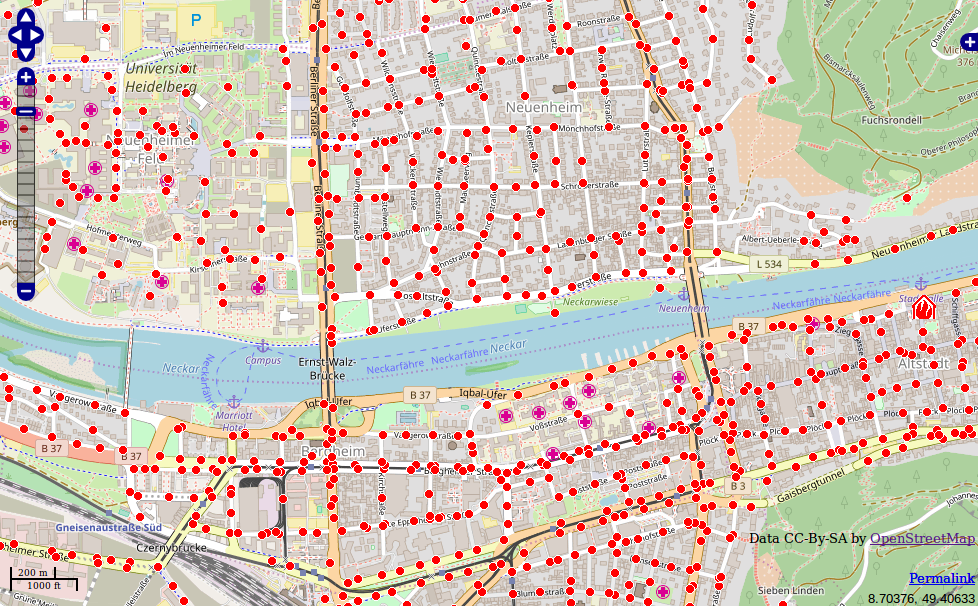
\includegraphics[width = 0.80 \textwidth]{../media/firehydrants.png} \\
\end{figure}

Das Analysieren der Teststrecken ist durch das einzelne Senden der Requests und das anschließende Extrahieren der benötigten Werte zeitaufwändig.
Es wäre demnach hilfreich ein Service zum gleichzeitigen senden von allen Testrequests zu entwickeln mit welchem danach ebenso die Antworten adäquat dargestellt werden können.
Dabei sollten zum Beispiel die Distanzen zwischen wichtigen Änderungspunkten auf einer Route berechnet werden können und tabellarisch aufgelistet werden.

Ein weiterer interessanter Aspekt den es zu beleuchten gilt, ist das unterschiedliche Verkehrsaufkommen auf einer Straße oder Fußgängerzone.
So könnten Geschwindigkeiten für bestimmte Wegsegmente je nach Zeit anhand von Berufsverkehr oder Tageszeit angepasst werden.
Nachts sollten beispielsweise generell weniger Autos auf der Straße sein, wodurch Zeit gespart wird, umgekehrt zum Berufsverkehr.

Die im Fragebogen erwähnte Suche nach Löschwasser Quellen am Zielort kann und sollte verwirklicht werden.
In der \gls{osm}-Datengrundlage existieren bereits diverse Tags für Objekte, die von Einsatzkräften genutzt werden können.
Für die Feuerwehr besonders interessant ist zum Beispiel der \texttt{emergency=fire\_hydrant} Tag für Hydranten.
In vielen Städten sind diese durch das OpenFireMap-Projekt\footnote{https://wiki.openstreetmap.org/wiki/DE:OpenFireMap} flächendeckend digitalisiert und der \gls{osm}-Datenbank zur Verfügung gestellt worden (Abb.~\ref{fig:firehydrants}).